\documentclass[12pt]{article}

\usepackage{graphicx}
\usepackage{amsmath}

\begin{document}

\section{Least-squares fitting}

\subsection{Model}

\begin{equation}
y=\alpha_{0}+\alpha_{1}x
\end{equation}

\subsection{Data}

\begin{table}[ht]
\begin{centering}
\begin{tabular}{ccc}
i & $x_{i}$ & $y_{i}$\\
1 & 0 & 0 \\
2 & 2 & 3 \\
3 & 4 & 5 \\
\end{tabular}
\par\end{centering}
\caption{Data.}
\end{table}

\begin{figure}[ht]
\begin{centering}
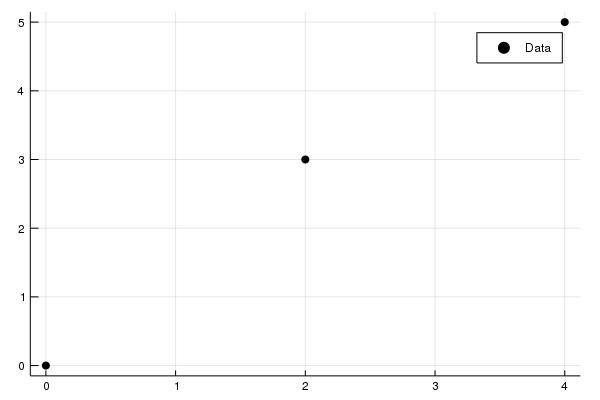
\includegraphics[width=\columnwidth]{data.png}
\end{centering}
\caption{Data.}
\end{figure}

\section{Solution}

\begin{align*}
\alpha_{0}+\alpha_{1}0 & =0\\
\alpha_{0}+\alpha_{1}2 & =3\\
\alpha_{0}+\alpha_{1}4 & =5
\end{align*}


\[
\left[\begin{array}{cc}
1 & 0\\
1 & 2\\
1 & 4
\end{array}\right]\left[\begin{array}{c}
\alpha_{0}\\
\alpha_{1}
\end{array}\right]=\left[\begin{array}{c}
0\\
3\\
5
\end{array}\right]
\]

\begin{align*}
\boldsymbol{X}\boldsymbol{\alpha} & =\boldsymbol{y}\qquad|\boldsymbol{X}^{\mathrm{T}}\cdot\left(\cdot\right)\\
\boldsymbol{X}^{\mathrm{T}}\boldsymbol{X}\boldsymbol{\alpha} & =\boldsymbol{X}^{\mathrm{T}}\boldsymbol{y}\qquad|\left(\boldsymbol{X}^{\mathrm{T}}\boldsymbol{X}\right)^{-1}\cdot\left(\cdot\right)\\
\boldsymbol{\alpha} & =\left(\boldsymbol{X}^{\mathrm{T}}\boldsymbol{X}\right)^{-1}\boldsymbol{X}^{\mathrm{T}}\boldsymbol{y}
\end{align*}

\begin{figure}[ht]
\begin{centering}
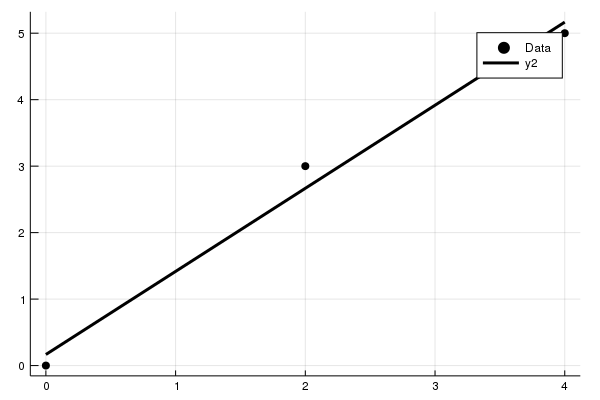
\includegraphics[width=\columnwidth]{solution.png}
\end{centering}
\caption{Solution.}
\end{figure}

\end{document}